

%----------------------------------------------------------------------------------------
%	PACKAGES AND OTHER DOCUMENT CONFIGURATIONS 
%----------------------------------------------------------------------------------------

\documentclass[paper=a4, fontsize=11pt]{scrartcl} % A4 paper and 11pt font size

\usepackage[T1]{fontenc} % Use 8-bit encoding that has 256 glyphs
\usepackage{fourier} % Use the Adobe Utopia font for the document - comment this line to return to the LaTeX default
\usepackage[english]{babel} % English language/hyphenation
\usepackage{amsmath,amsfonts,amsthm} % Math packages

\usepackage{lipsum} % Used for inserting dummy 'Lorem ipsum' text into the template

\usepackage{sectsty} % Allows customizing section commands
\allsectionsfont{\centering \normalfont\scshape} % Make all sections centered, the default font and small caps

\usepackage{graphicx}

\usepackage{fancyhdr} % Custom headers and footers
\pagestyle{fancyplain} % Makes all pages in the document conform to the custom headers and footers
\fancyhead{} % No page header - if you want one, create it in the same way as the footers below
\fancyfoot[L]{} % Empty left footer
\fancyfoot[C]{} % Empty center footer
\fancyfoot[R]{\thepage} % Page numbering for right footer
\renewcommand{\headrulewidth}{0pt} % Remove header underlines
\renewcommand{\footrulewidth}{0pt} % Remove footer underlines
\setlength{\headheight}{13.6pt} % Customize the height of the header

\numberwithin{equation}{section} % Number equations within sections (i.e. 1.1, 1.2, 2.1, 2.2 instead of 1, 2, 3, 4)
\numberwithin{figure}{section} % Number figures within sections (i.e. 1.1, 1.2, 2.1, 2.2 instead of 1, 2, 3, 4)
\numberwithin{table}{section} % Number tables within sections (i.e. 1.1, 1.2, 2.1, 2.2 instead of 1, 2, 3, 4)

\setlength\parindent{0pt} % Removes all indentation from paragraphs - comment this line for an assignment with lots of text

%----------------------------------------------------------------------------------------
%	TITLE SECTION
%----------------------------------------------------------------------------------------

\newcommand{\horrule}[1]{\rule{\linewidth}{#1}} % Create horizontal rule command with 1 argument of height

\title{	
\normalfont \normalsize 
\textsc{Software Engineering ELEN4009} \\ [25pt] % Your university, school and/or department name(s)
\horrule{0.5pt} \\[0.4cm] % Thin top horizontal rule
\huge LABORATORY EXERCISE 3 \\ % The assignment title
\horrule{2pt} \\[0.5cm] % Thick bottom horizontal rule
}

\author{ Sheena Philip, Linda Khumalo, Kessigan Subramanium, Phumzile Dhlwathi} % Your name

\date{\normalsize\today} % Today's date or a custom date

\begin{document}

\maketitle % Print the title

%----------------------------------------------------------------------------------------
%	PROBLEM 1
%----------------------------------------------------------------------------------------

\section{User Manual}

\subsection{Necessary information to check repo on GitHub}
\begin{itemize}
\item Go to: github.com/kessigan/Transport\_System
\item clone the repo
\item Go to the folder Lab3/Project
\end{itemize}

\subsection{Softwares To Install}
\begin{itemize}
\item  Install Anaconda python 2.7
\item django 1.9.4
\item postgresql 9.5.1 - the password is "password" the user is "postgres"
\item psycopg2-2.6.1
\item pgadminIII

\end{itemize}

\subsection{Set-up before the project is run}
\begin{itemize}
\item make the database
\begin{itemize}
\item Go to pgAdminIII
\item log in to the postgres server
\item right click on Databases
\item select New Database
\item under Name, type MainDB
\item click OK - a database is now created

\end{itemize}
\end{itemize}

\subsection{Description of how to compile code}
\begin{itemize}
\item Go to the folder Lab3/Project/CourierJZ
\item type : python createDatabases.py . The user has now added three tables to the MainDB created earlier.
\item Go to the folder Lab3/Project/CourierJZ
\item open terminal in this location
\item type : python manage.py runserver . Django server is now running
\item Go to browser (preferably Chrome). Type in localhost:8000/courier/main

 

\end{itemize}

\subsection{Description of the front end}
In order to use the service the user first needs view the main page. This page is located at localhost:8000/courier/main. From this page the user is able to select their designation, the four options available are driver, sender, receiver and dispatcher. The user will then need to submit their login details, for this version the super-user email is admin and the password is also admin. At this stage the sender is able to fill a form to send a package, the receiver is able to submit a form to see the package status, the dispatcher is able to see the current packages that remain in the warehouse and the driver is able to see a map of the area he is in as well as the list of packages to be picked up or dropped off.

\section{Description of project}

\subsection{PROBLEM STATEMENT}

Courier JZ currently uses an inefficient, time consuming, tedious system which is not centralised or automated to manage their fleet of delivery and pick-up vehicles.


%%%%%%%%%%%%%%%%%%%%%%%%%%%%%%%%%%%%%%%%%%%%%%%%%%%%%%%%%%%%%%%%%%%%%%%%%%%%%%%
%
\subsection{PROJECT OBJECTIVES}

\begin{itemize}
\item To design, implement and test a web-based management system for a fleet of delivery and pick-up vehicles
\item The website must serves as a platform to integrate the various activities of the personnel involved in the day to day running of the business
\item The website must automate previously time-consuming activities resulting in a  more efficient company.
\item The website must act as a repository  to store all the data associated with the business activities.
\end{itemize}

\subsection{Current Implementation of Project}

A prototype of the project has been created thus far. The following features have been implemented in terms of their front-end


\subsubsection{The driver interface/view}
 Figure 2.1 displays the view of the driver. The current prototype has deviated from the designed view in that the estimated time of arrival does not appear and the client contact details do not appear.
\begin{figure}[hbt!]
\centering
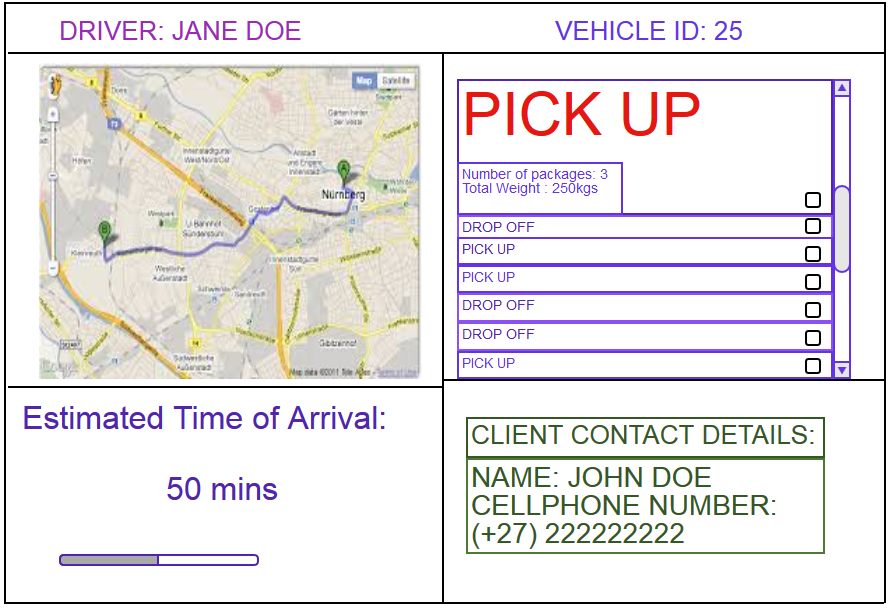
\includegraphics[width=5in]{screenshots/driver.png}
\caption{The driver interface}
\label{Driver}
\end{figure}

\subsubsection{The dispatcher view}
Figure 2.2 displays the dispatcher view before the dispatcher runs the algorithm to assign packages to drivers and routes. The current prototype achieves this view.
\begin{figure}[hbt!]
\centering
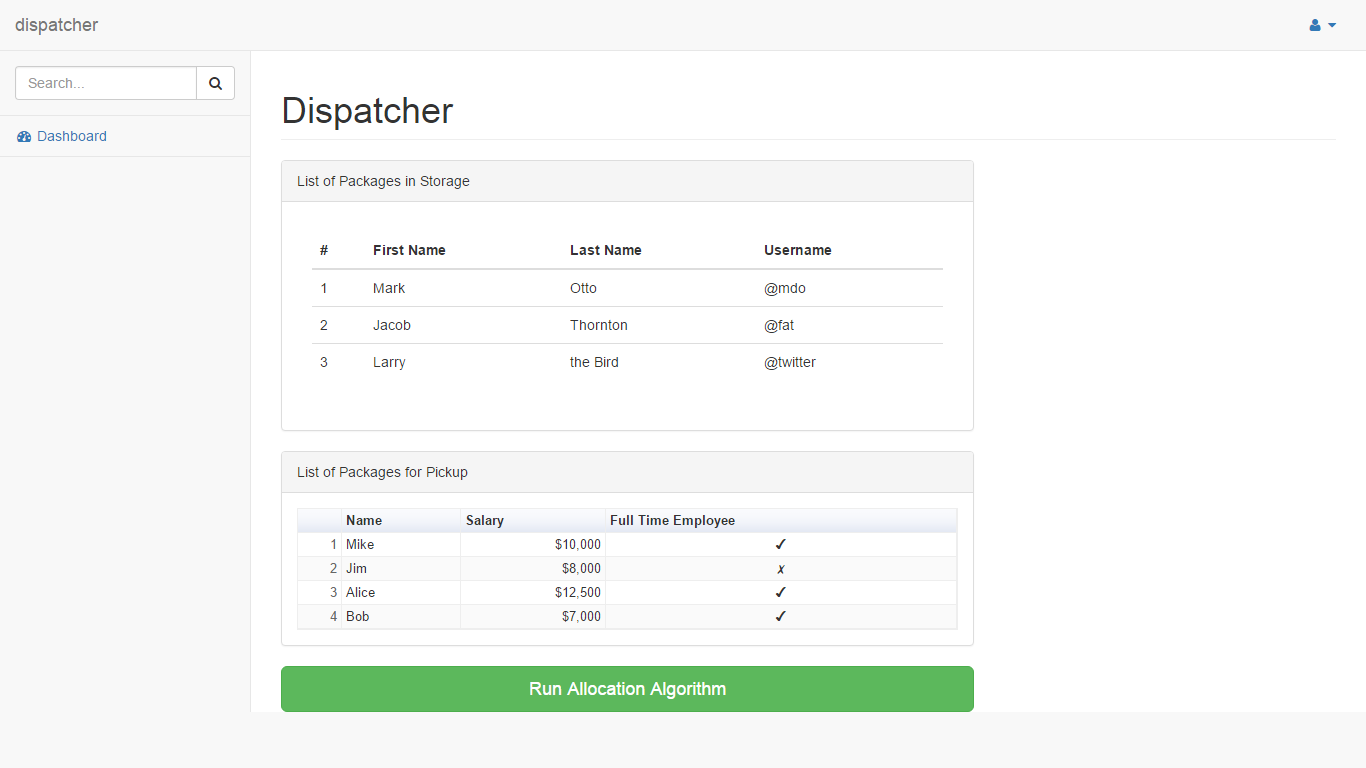
\includegraphics[width=5in]{screenshots/dispatcher.png}
\caption{The dispatcher interface before running the allocation algorithm}
\label{DispatcherBefore}
\end{figure}

\subsubsection{The receiver view before user submits}
In order for the receiver to track the progress of their package they have to enter the package ID sent to them via email notification. Figure \ref{ReceiverBefore} shows the page where the user enters their package id. The current prototype achieves this view.
\begin{figure}[hbt!]
\centering
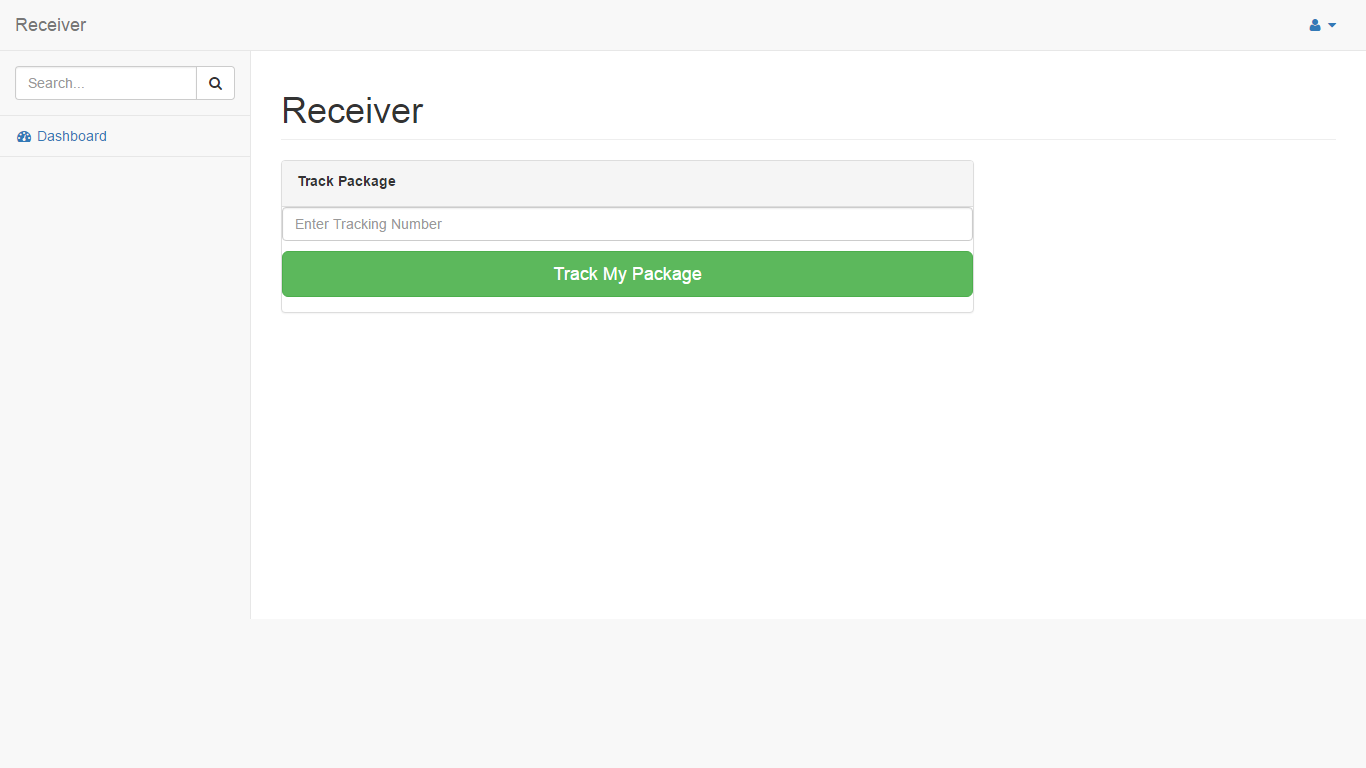
\includegraphics[width=5in]{screenshots/receiver.png}
\caption{The receiver interface}
\label{ReceiverBefore}
\end{figure}


\subsubsection{The sender view}
Figure \ref{Sender} shows the sender view. 
\begin{figure}[hbt!]
\centering
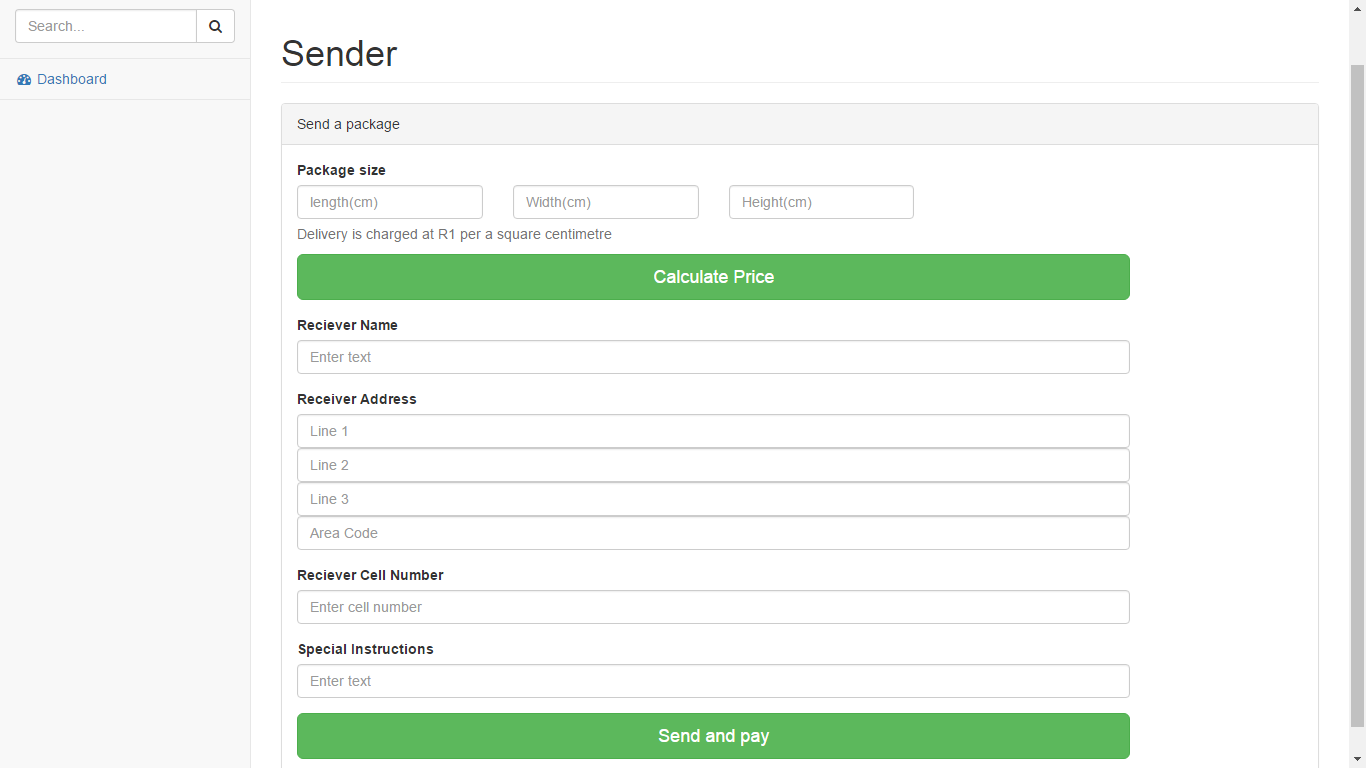
\includegraphics[width=5in]{screenshots/sender.png}
\caption{The sender interface}
\label{Sender}
\end{figure}

\break

The back-end is used to store and process all information as requested by the users. In its current form of the project the user information is stored on the database, information may be added to the database from form submissions on the user pages, this includes the submission of a pick-up requests with the relevant delivery details and the user been able to track a package. The information is sent from the webpage to the server. The server then processes the data and returns user specific information.


\section{Current implementation responsibility of each pair of students}

\subsection{	BACK--END : Linda, Phumzile}


\begin{itemize}
	\item  make a database and populate it - Linda
	\item  implement algorithms which can calculate things related to the front end, such as:
		\begin{itemize}
		\item packing algorithm - Phumzile
		\end{itemize}
	\item set up a server		- Phumzile
	\item link database to server	- Linda
	\item	link front end to server - Linda

\end{itemize}


\subsection{	FRONT END : Kessigan, Sheena}

\begin{itemize}
	\item  Make user interfaces for the different users

		\begin{itemize}
		 \item Choose a bootstrap template and make minor modifications - Sheena
		
		\item Dispatcher (inputs the variables so the algorithms can run and return a result) - Kessigan
		\item Driver Page:		
			\begin{itemize} 
		\item location - Kessigan
																
					\item schedule	- Sheena
					\item goods transferred/pickup - Kessigan
					\item location - Sheena
		\end{itemize}
		
		\end{itemize}
	
	
\end{itemize}


%----------------------------------------------------------------------------------------

\end{document}